%  Asym.tex
%  Document created by seblovett on seblovett-Ubuntu
%  Date created: Mon 31 Mar 2014 11:50:09 BST
%  <+Last Edited: Mon 31 Mar 2014 21:03:13 BST by seblovett on seblovett-Ubuntu +>

\section{Asymmetric Multi-Cores}

\subsection{Theory}
\todo[inline]{get buzz word `hetrogeneous' in here a few times}
Discuss symmetric, performance asymmetric and asymmetric multi-cores
Multi-core architectures are not a new concept. 
A multi-core processor is a single die with two or more independent identical CPUs. 
They can have a shared cache and be connected on a bus.
An asymmetric multi-core processor is a chip which has two or more independent CPUs (usually two).
The difference to a symmetric multi-core processor, is that the cores are not the same. 
The cores can differ in cache, clock frequency, area and power, but maintain the same Instruction Set Architecture \cite{de2012power}.
The cores therefore can have different optimisations.


Asymmetric multi-core architectures can be split into two categories - function or performance asymmetry \cite{wang2012energy}.
Performance asymmetry is where the cores differ only by their performance, and subsequently power. 
This is achieved by having a multi-core processor with cores that can be individually gated, or scaled with DVFS.
The Intel Single-chip Cloud Computer is such a device that supports this \cite{IntelSCC}.

Functional asymmetry is where the processor has heterogeneous with memory, architecture (and usually also performance).
One large upcoming functional asymmetric multi-core architecture is the ARM big.LITTLE. 
The architecture of the device is seen in figure \ref{fig:bigLITTLE:arch}.
There are two cores in the big.LITTLE - a Cortex A15 and Cortex A7.
The A15 is a high performance, high energy consumption, out of order execution processor.\todo{discuss cache differences}
The A7 is the opposite of the A15 as it is an in order, energy efficient processor, and a compromise of performance.
This asymmetric configuration allows performance critical tasks to be performed on the larger core, which can be powered down during periods of inactivity while the smaller, energy efficient core conducts other, non performance reliant tasks.
big.LITTLE implements clock and power gating, and Dynamic Voltage and Frequency Scaling on the cores to aid the energy savings.


\begin{figure}
%missingfigure{ARM big.LITTLE architecture}
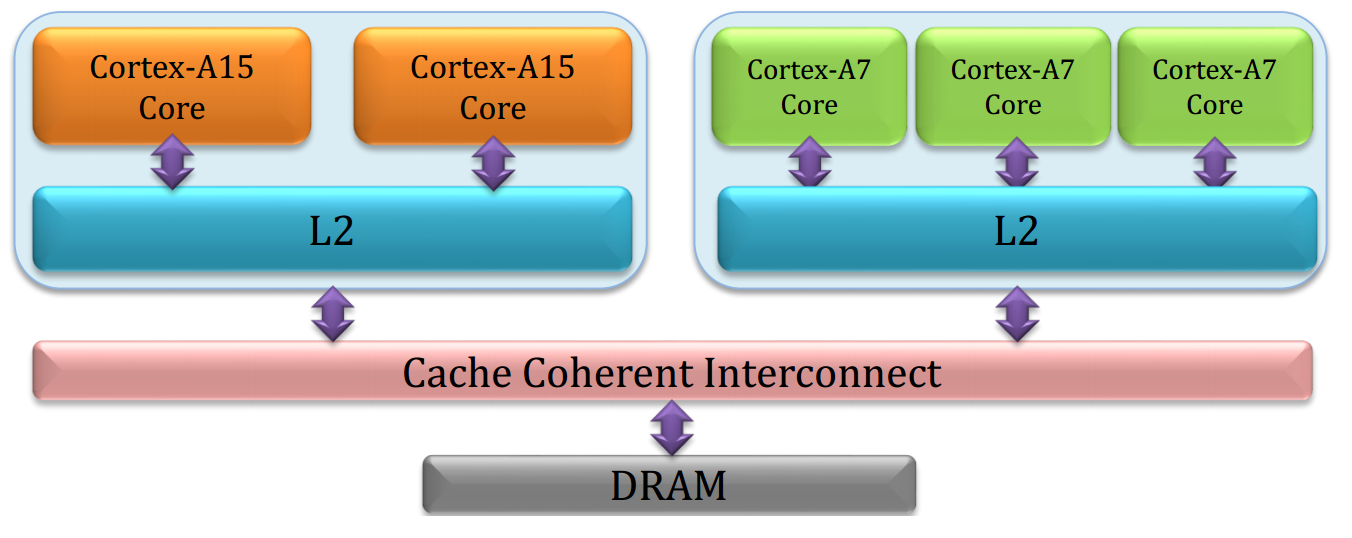
\includegraphics[width=0.45\textwidth]{Figures/armbiglittle.png}
\caption{ARM big.LITTLE Architecture diagram, from \cite{muthukaruppan2013hierarchical}.}
\label{fig:bigLITTLE:arch}
\end{figure}

\todo[inline]{Discuss pros/cons to AMC}

\subsection{Scheduling Techniques}

The main issue to asymmetric multi-core architectures is around the scheduling of tasks to the correct core.
Parallel programming also is not directly applicable to a asymmetric architecture. 
This is due to the assumption of symmetry in parallel programming - that each task would take the same time on any core. 
This is not so due to the performance difference between the cores.

%\cite{esmaeilzadeh2011dark,jimenez2009predictive} Idea of small core getting memory intensive. Primitive but a start.
A primitive, but reasonable, scheduler is outlined in \cite{esmaeilzadeh2011dark} and \cite{jimenez2009predictive}.
Here, a hard fast allocation is made. 
Memory intensive workloads are given to the small core and computationally heavy tasks are allocated to the larger core. 
This is beneficial as memory intensive tasks are generally slow due to the access delays to the memory. 
However, with varying sizes of caches between the architectures, this method is suboptimal. 
A more in-depth method is necessary, looking at more than compile time directives.


%RUN TIME SCHEDULING
%\cite{chen2012wats} task stealing, performance optimisation.
%\cite{de2012power} run time to decide on thread scheduling, clock gating and DVFS

Run time can provide useful information of the tasks. 
\cite{chen2012wats} proposes a scheduler for an asymmetric multi-core processor which uses the history of the tasks to allocate which core to schedule to. % leading to a near optimal solution.
A task stealing policy is also implemented. 
This allows the bigger core to take over a task from the smaller core if it takes a long time.
Task stealing is also scalable. 
\cite{chen2012wats} showed that their algorithm gave an 82.7\% increase in the performance of the processor by using history based scheduling.

%HIGH LEVEL
%\cite{zhu2013high} - uses two chips (A9 and A8} to look at mobile browsing.
%\cite{wang2012energy} scheduling of VMs. Higher level of scheduler, but shows promise.
Scheduling can also be done at a higher level. 
\cite{zhu2013high} looks a popular mobile task - web browsing. 
Parsing web pages can take varying amounts of time, but are generally very complex tasks. 
An asymmetric multi-core set up is used using an ARM Cortex A9 for the `big' core and an A8 for the 'little' core. 
It shows that even at a high level of task, a big/little configuration can yield energy savings without a drastic performance decrease compared to performance focussed systems.

Virtual machines (VMs) are commonly used on servers. 
Some VMs can perform intensive tasks, where others do not need large performance capabilities.
However, it can be difficult to predict when and if a VM needs performance, as the applications run may not be known to the host. 
\cite{wang2012energy} proposes a task scheduler for use on an asymmetric multi-core. 
Current schedulers are not aware of the heterogeneities of the processor cores. 
The scheduling algorithm here uses only run time characteristics of the virtual machine, but achieves between 13.5\% and 55\% increase in performance per watt.

A combination of compile time and run time can aid optimisations further. 
\cite{de2012power} gives a brief overview of using these measurements to the tread scheduling as well as lower level energy saving aspects such as clock gating and DVFS. 

%VERY GOOD ONES
%\cite{pricopi2013power} has a measure, looks at compile time and run time. Measures for one, estimates for other and decides if need to schedule differently.

In the ARM big.LITTLE architecture, the two cores differ greatly. 
Not only the frequency of the core is different, but there are differing numbers of pipeline stages, cache sizes and branch predictions.
The A15 also has cache miss and branch misprediction counters, where as the A8 does not. 
The main thing the two cores have in common is that they share the same instruction set. 
Due to the differences of the cores, it is difficult to predict the performance of a task on a core.
One technique used is looking at the Cycles per instruction of the core \cite{pricopi2013power}. 
This gives an insight into the differences of the cores. 
This measure can then be used to predict the power consumption of the task when run on the other core. 
However, this is unable to identify data dependencies of the task. 
Compile time directives are therefore used to help predict stalls in the pipeline. 


%\cite{muthukaruppan2013hierarchical} - big.LITTLE used. Minimising energy consumption (not just increasing performance). power budget. 
Performance and energy consumption are not the only things to be considered on a low energy core.
The thermal characteristics can also be important, especially in mobile devices where cooling is not generally available. 
\cite{muthukaruppan2013hierarchical} suggests a scheduler where the large core is used sparingly, and all cores are run at minimum frequency when possible. 
A power budget is implemented here also, which is to reduce the thermal expenditure of the device. 
If the power budget is spent, then the performance of the device is lowered until it is possible to recover. 
This concept is a different view on the energy consumption, but involves solving the same problem. 


\subsection{Conclusion}

%\todo[inline]{Good or bad idea? Have the issues been solved?}

Asymmetric multi-core architectures are very promising to achieving a good compromise between the performance and energy consumption of a processor. 
The main issue that this architecture faces is correctly scheduling the tasks to the correct cores. 
If the allocation is sub-optimal, then the asymmetry will be a hindrance to the processor. 
It has been shown, however, that correct task allocation results in energy savings, compared to non-symmetric architectures. 
The scheduling can be done purely on run time statistics to a satisfactory level, but by utilising hardware counters available and compile time directives, the energy savings can be much larger.
